\chapter{Formal Concept Analysis}
\label{chapter:formal-concept-analysis}

Formal Concept Analysis (FCA) provides a simple, and yet mathematically rigorous, framework for identifying and reasoning about ``concepts'' and their corresponding hierarchies in data \cite{ganter1999formal,ganter2016conceptual}. Its central view of concepts as a dual between \textit{extension}---what one refers to as instances of a concept---and \textit{intension}---what meaning is ascribed to a concept---is supported by a rich philosophical backing. \index{formal concept analysis}

\section{Basic Notions}
\label{section:basic-notions}
The `atoms' in FCA are given by \textit{objects} and \textit{attributes}; objects relate to extension, and attributes to intension. These are unified under a structure called a \textit{formal context}.

\begin{definition}
  \label{definition:formal-context}
  A \textbf{formal context} $\Fcontext$ is a triple comprised of a set of objects $G$, a set of attributes $M$, and a binary relation $I \; \subseteq G \times M$ referred to as an `incidence' relation. For an object-attribute pair $(g,m) \in I$ we say that \say{object $g$ \textit{has} the attribute $m$}.
\end{definition}

A formal context \index{formal context} in some sense describes an open-world interpretation, and so $(g,m) \not \in I$ is not usually interpreted as saying that \say{object $g$ has the negation of the attribute $m$}.

\begin{example}
  \label{example:first-example-formal-context}
  Formal contexts of reasonable size can be described entirely by a matrix-like representation. Each object corresponds to a row, and each attribute to a column.

  \begin{figure}[H]
    \centering
    \scriptsize
    \begin{tabular}{|c||c|c|c|c|c|}
      \hline
      & \rotatebox{0}{\texttt{closure}}
      & \rotatebox{0}{\texttt{associativity}}
      & \rotatebox{0}{\texttt{identity}}
      & \rotatebox{0}{\texttt{divisibility}}
      & \rotatebox{0}{\texttt{commutativity}} \\
      \hline\hline
      \texttt{magma}             & $\times$ &          &          &          &          \\ \hline
      \texttt{semigroup}         & $\times$ & $\times$ &          &          &          \\ \hline
      \texttt{monoid}            & $\times$ & $\times$ & $\times$ &          &          \\ \hline
      \texttt{group}             & $\times$ & $\times$ & $\times$ & $\times$ &          \\ \hline
      \texttt{abelian group}     & $\times$ & $\times$ & $\times$ & $\times$ & $\times$ \\ \hline
      \texttt{loop}              & $\times$ &          & $\times$ & $\times$ &          \\ \hline
      \texttt{quasigroup}        & $\times$ &          &          & $\times$ &          \\ \hline
      \texttt{groupoid}          &          & $\times$ & $\times$ & $\times$ &          \\ \hline
      \texttt{category}          &          & $\times$ & $\times$ &          &          \\ \hline
      \texttt{semicategory}      &          & $\times$ &          &          &          \\ \hline
      \specialrule{1.25pt}{0pt}{0pt}
    \end{tabular}
    \caption{A formal context showing necessary properties of group-like structures.}
    \label{figure:formal-context-group-structures}
  \end{figure}
\end{example}

A formal

\begin{figure}[H]
  \centering
  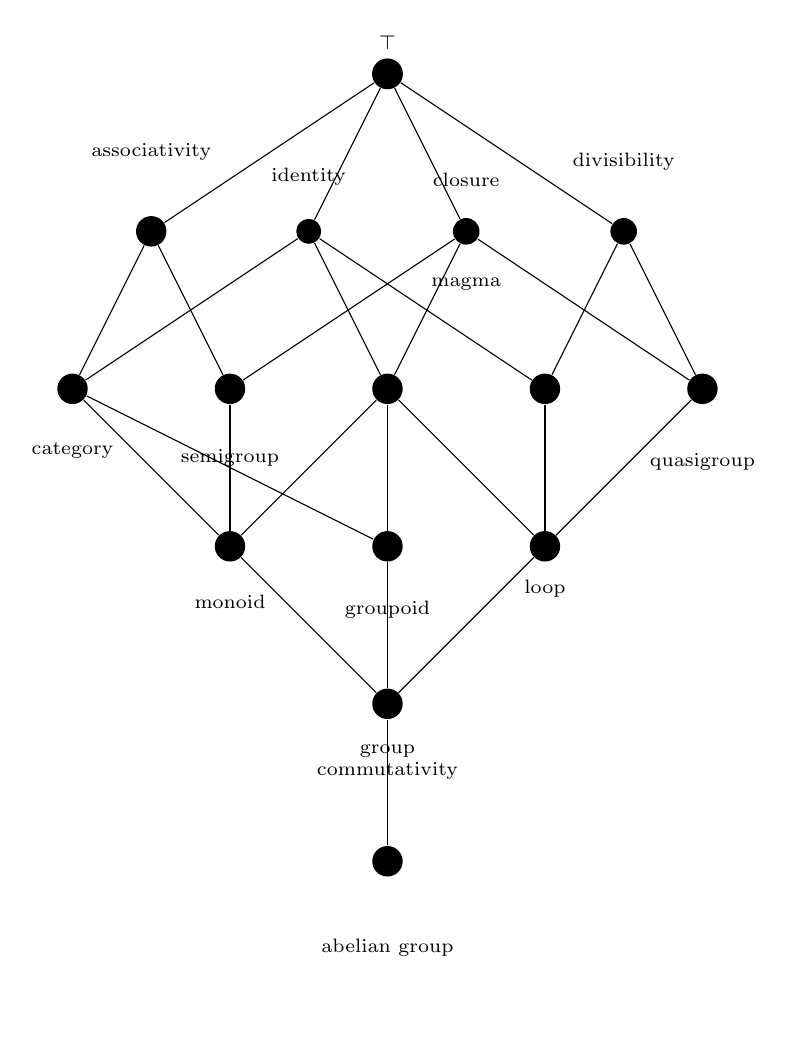
\begin{tikzpicture}[every node/.style={circle, fill=black, inner sep=1pt}]
    \node (a1) at (0,3) [label=above:{\scriptsize $\top$}] {w};
    % \node[draw=none, fill=none] at (0,3.5) {\tiny Top};

    \node (b1) at (-3,1) [label=above:{\scriptsize associativity}] {y};
    \draw (a1) -- (b1);

    \node (b2) at (-1,1) [label=above:{\scriptsize identity}] {z};
    \draw (a1) -- (b2);

    \node (b3) at (1,1) [label=above:{\scriptsize closure},label=below:{\scriptsize magma}] {x};
    \draw (a1) -- (b3);

    \node (b4) at (3,1) [label=above:{\scriptsize divisibility}] {x};
    \draw (a1) -- (b4);

    \node (c1) at (-4,-1) [label=below:{\scriptsize category}] {y};
    \draw (c1) -- (b1);
    \draw (c1) -- (b2);

    \node (c2) at (-2,-1) [label=below:{\scriptsize semigroup}] {y};
    \draw (c2) -- (b1);
    \draw (c2) -- (b3);

    \node (c3) at (0,-1) {y};
    \draw (c3) -- (b2);
    \draw (c3) -- (b3);

    \node (c4) at (2,-1) {y};
    \draw (c4) -- (b2);
    \draw (c4) -- (b4);

    \node (c5) at (4,-1) [label=below:{\scriptsize quasigroup}] {y};
    \draw (c5) -- (b3);
    \draw (c5) -- (b4);

    \node (d1) at (-2,-3) [label=below:{\scriptsize monoid}] {y};
    \draw (d1) -- (c1);
    \draw (d1) -- (c2);
    \draw (d1) -- (c3);

    \node (d2) at (0,-3) [label=below:{\scriptsize groupoid}] {y};
    \draw (d2) -- (c1);
    \draw (d2) -- (c3);

    \node (d3) at (2,-3) [label=below:{\scriptsize loop}] {y};
    \draw (d3) -- (c3);
    \draw (d3) -- (c4);
    \draw (d3) -- (c5);

    \node (e1) at (0,-5) [label=below:{\scriptsize group}] {y};
    \draw (e1) -- (d1);
    \draw (e1) -- (d2);
    \draw (e1) -- (d3);

    \node (f1) at (0,-7)[label=above:{\scriptsize commutativity},label=below:{\scriptsize abelian group}] {y};
    \draw (f1) -- (e1);
  \end{tikzpicture}
  \caption{The concept lattice associated with the formal context in \Cref{figure:formal-context-group-structures}}
\end{figure}